%%
%% This is file `sample-xelatex.tex',
%% generated with the docstrip utility.
%%
%% The original source files were:
%%
%% samples.dtx  (with options: `sigconf')
%% 
%% IMPORTANT NOTICE:
%% 
%% For the copyright see the source file.
%% 
%% Any modified versions of this file must be renamed
%% with new filenames distinct from sample-xelatex.tex.
%% 
%% For distribution of the original source see the terms
%% for copying and modification in the file samples.dtx.
%% 
%% This generated file may be distributed as long as the
%% original source files, as listed above, are part of the
%% same distribution. (The sources need not necessarily be
%% in the same archive or directory.)
%%
%% Commands for TeXCount
%TC:macro \cite [option:text,text]
%TC:macro \citep [option:text,text]
%TC:macro \citet [option:text,text]
%TC:envir table 0 1
%TC:envir table* 0 1
%TC:envir tabular [ignore] word
%TC:envir displaymath 0 word
%TC:envir math 0 word
%TC:envir comment 0 0
%%
%%
%% The first command in your LaTeX source must be the \documentclass command.
\PassOptionsToPackage{table}{xcolor}
\documentclass[sigconf,nonacm]{acmart}
%% NOTE that a single column version is required for 
%% submission and peer review. This can be done by changing
%% the \doucmentclass[...]{acmart} in this template to 
%% \documentclass[manuscript,screen]{acmart}
%% 
%% To ensure 100% compatibility, please check the white list of
%% approved LaTeX packages to be used with the Master Article Template at
%% https://www.acm.org/publications/taps/whitelist-of-latex-packages 
%% before creating your document. The white list page provides 
%% information on how to submit additional LaTeX packages for 
%% review and adoption.
%% Fonts used in the template cannot be substituted; margin 
%% adjustments are not allowed.

%%
%% \BibTeX command to typeset BibTeX logo in the docs
\AtBeginDocument{%
  \providecommand\BibTeX{{%
    \normalfont B\kern-0.5em{\scshape i\kern-0.25em b}\kern-0.8em\TeX}}}

%% Rights management information.  This information is sent to you
%% when you complete the rights form.  These commands have SAMPLE
%% values in them; it is your responsibility as an author to replace
%% the commands and values with those provided to you when you
%% complete the rights form.
% \setcopyright{acmcopyright}
% \copyrightyear{2018}
% \acmYear{2018}
% \acmDOI{XXXXXXX.XXXXXXX}

%% These commands are for a PROCEEDINGS abstract or paper.
% \acmConference[Conference acronym 'XX]{Make sure to enter the correct
%   conference title from your rights confirmation emai}{June 03--05,
%   2018}{Woodstock, NY}
%
%  Uncomment \acmBooktitle if th title of the proceedings is different
%  from ``Proceedings of ...''!
%
%\acmBooktitle{Woodstock '18: ACM Symposium on Neural Gaze Detection,
%  June 03--05, 2018, Woodstock, NY} 
% \acmPrice{15.00}
% \acmISBN{978-1-4503-XXXX-X/18/06}

\usepackage[table]{xcolor}
\usepackage{array}
\usepackage{xeCJK}
\usepackage{multirow}
\setCJKmainfont[AutoFakeBold=true, AutoFakeSlant=true]{標楷體}

\newcolumntype{P}[1]{>{\raggedright\vrule height4ex width 0pt}p{#1}<{\vrule depth 2.5ex width 0pt}}


%%
%% Submission ID.
%% Use this when submitting an article to a sponsored event. You'll
%% receive a unique submission ID from the organizers
%% of the event, and this ID should be used as the parameter to this command.
%%\acmSubmissionID{123-A56-BU3}

%%
%% The majority of ACM publications use numbered citations and
%% references.  The command \citestyle{authoryear} switches to the
%% "author year" style.
%%
%% If you are preparing content for an event
%% sponsored by ACM SIGGRAPH, you must use the "author year" style of
%% citations and references.
%% Uncommenting
%% the next command will enable that style.
%%\citestyle{acmauthoryear}
%%
%% end of the preamble, start of the body of the document source.
\begin{document}

%%
%% The "title" command has an optional parameter,
%% allowing the author to define a "short title" to be used in page headers.
\title{Accelerate Canny Edge Detector with Parallel Programming}

%%
%% The "author" command and its associated commands are used to define
%% the authors and their affiliations.
%% Of note is the shared affiliation of the first two authors, and the
%% "authornote" and "authornotemark" commands
%% used to denote shared contribution to the research.
\author{Zi Yi Huang}
\affiliation{
  \institution{312551072}
  \institution{IOC, NYCU}
  \city{Hsinchu}
  \country{Taiwan}
}
\email{m312551072.cs12@nycu.edu.tw}

\author{Bo Han Chen}
\affiliation{
  \institution{312551074}
  \institution{IOC, NYCU}
  \city{Hsinchu}
  \country{Taiwan}
}
\email{bhchen312551074.cs12@nycu.edu.tw}

\author{Hsuan Yu Chi}
\affiliation{
  \institution{312551080}
  \institution{IOC, NYCU}
  \city{Hsinchu}
  \country{Taiwan}
}
\email{chihy.cs12@nycu.edu.tw}

%%
%% By default, the full list of authors will be used in the page
%% headers. Often, this list is too long, and will overlap
%% other information printed in the page headers. This command allows
%% the author to define a more concise list
%% of authors' names for this purpose.
% \renewcommand{\shortauthors}{Trovato and Tobin, et al.}

%%
%% The abstract is a short summary of the work to be presented in the
%% article.
\begin{abstract}
  本報告中,我們利用不同的平行化 API 加速 Canny Edge Detection 演算法,分析各個步驟的最佳平行化方式,
  並比較了在不同圖片尺寸下的執行時間與使用不同數量的 thread 的 speedup。
\end{abstract}

%%
%% The code below is generated by the tool at http://dl.acm.org/ccs.cfm.
%% Please copy and paste the code instead of the example below.
%%
% \begin{CCSXML}
% <ccs2012>
%  <concept>
%   <concept_id>00000000.0000000.0000000</concept_id>
%   <concept_desc>Do Not Use This Code, Generate the Correct Terms for Your Paper</concept_desc>
%   <concept_significance>500</concept_significance>
%  </concept>
%  <concept>
%   <concept_id>00000000.00000000.00000000</concept_id>
%   <concept_desc>Do Not Use This Code, Generate the Correct Terms for Your Paper</concept_desc>
%   <concept_significance>300</concept_significance>
%  </concept>
%  <concept>
%   <concept_id>00000000.00000000.00000000</concept_id>
%   <concept_desc>Do Not Use This Code, Generate the Correct Terms for Your Paper</concept_desc>
%   <concept_significance>100</concept_significance>
%  </concept>
%  <concept>
%   <concept_id>00000000.00000000.00000000</concept_id>
%   <concept_desc>Do Not Use This Code, Generate the Correct Terms for Your Paper</concept_desc>
%   <concept_significance>100</concept_significance>
%  </concept>
% </ccs2012>
% \end{CCSXML}

% \ccsdesc[500]{Do Not Use This Code~Generate the Correct Terms for Your Paper}
% \ccsdesc[300]{Do Not Use This Code~Generate the Correct Terms for Your Paper}
% \ccsdesc{Do Not Use This Code~Generate the Correct Terms for Your Paper}
% \ccsdesc[100]{Do Not Use This Code~Generate the Correct Terms for Your Paper}

%%
%% Keywords. The author(s) should pick words that accurately describe
%% the work being presented. Separate the keywords with commas.
% \keywords{Do, Not, Us, This, Code, Put, the, Correct, Terms, for,
%   Your, Paper}

%% A "teaser" image appears between the author and affiliation
%% information and the body of the document, and typically spans the
%% page.
% \begin{teaserfigure}
%   \includegraphics[width=\textwidth]{sampleteaser}
%   \caption{Seattle Mariners at Spring Training, 2010.}
%   \Description{Enjoying the baseball game from the third-base
%   seats. Ichiro Suzuki preparing to bat.}
%   \label{fig:teaser}
% \end{teaserfigure}

% \received{20 February 2007}
% \received[revised]{12 March 2009}
% \received[accepted]{5 June 2009}

%%
%% This command processes the author and affiliation and title
%% information and builds the first part of the formatted document.
\maketitle

\section{Introduction}
  Canny Edge Detection (CED) 是一種常見的影像處理演算法,用於偵測圖片中的大範圍邊界。
  它是在1986年由John F. Canny發明。Canny Edge Detection可以有效地去除影像中的雜訊、
  模糊的邊緣與非邊緣的線,產生更高SNR的影像,使結果更為精細。
  以下是Canny Edge Detection常見的應用領域 (1) Object detection : 偵測影像中物體的邊緣,
  用於辨識物體。如用於偵測道路交通中的汽車、行人和其他物體。(2) Image segmentation : 
  將影像分割成不同的圖像子區域,用於進一步分析。實際可應用於醫學影像、指紋識別、人臉識別等 
  (3) Feature extraction : 從影像中提取特徵,提取物體的邊緣或建築物的角落。
  這些功能隨後可用於物件辨識。如從臉部影像提取特徵進行人臉識別,或從街道影像中提取特徵用於自動駕駛。
  結合以上應用,因此Canny Edge Detection在醫學圖像分析、機器人學、電腦視覺、
  工業檢驗相關研究領域廣泛使用。 \\
  Canny Edge Detection的優點可以分為以下幾點
  \begin{enumerate}
    \item Accurate edge localization : 可以精準的定位圖片中的邊緣,確保僅保留重要的邊緣。
    \item Low error rate : 演算法中double thresholding 與 edge tracking的機制降低誤判邊緣的可能性,
    因此有較低錯誤率。
    \item Single response to edges : 圖片中每條邊緣在輸出僅由single response表示,
    避免重複邊緣偵測,使線條更為細緻。
    \item Robust to noise : 適用於受到各種噪聲影響的真實世界圖片影像。
    起始步驟中的Smoothing使Canny Edge Detection具有很高的抗噪性。
  \end{enumerate}
  缺點則是
  \begin{enumerate}
    \item Computationally expensive : Canny Edge Detection的計算成本很高,尤其圖片解析度很高時。
    \item Sensitive to parameters : double thresholding的選擇會很大程度影響邊緣偵測的輸出結果,
    對於不同圖片會有適合的threshold。
  \end{enumerate}
  Canny Edge Detection的計算成本相當高,包含多個卷積、
  Gradient Computation、Nonmaxima Suppression、BFS搜尋。雖然複雜,
  但計算間有獨立性,可使用平行處理來加速。透過將影像劃分為多個區域,使用多個 thread
  平行處理每個區域,在多核心處理器上加速;或使用GPU來加速卷積運算。
  藉由平行運算,可以在不影響正確性的情形下提升計算效率與throughput,滿足需要處理大量資料的需求。

\section{Statement of Problem}

在這個部分,我們會介紹 Canny Edge Detection 演算法,描述演算法中各步驟的運作,
最後分析哪些部分是可以使用平行化來加速的。
Canny Edge Detection 演算法分成以下幾個步驟:Smoothing、Gradient Computation、
Nonmaxima Suppression、Double Thresholding 和 Hysteresis Edge Linking,
接下來我們會針對每個步驟做詳細的說明。

\subsection{Smoothing} \label{Smoothing}

對於 Smoothing,我們使用一個 $3\times3$ 的近似高斯濾波器 $G$ 來對輸入的影像進行卷積,
以達到平滑影像的效果。
$$G=\frac{1}{16}
\begin{bmatrix}
1 & 2 & 1 \\2 & 4 & 2 \\
1 & 2 & 1
\end{bmatrix}$$
令 $f(x, y)$ 為輸入影像,則經過 Smoothing 後的影像 $f_s(x, y)$ 可以表示為 $f$ 與 $G$ 的卷積,
如下算式所示:
$$f_s(x, y)=f(x, y)*G(x, y)$$

\subsection{Gradient Computation}

對於 Gradient Computation,我們需要計算上一步中得到的 $f_s(x, y)$ 上每個點的梯度大小與方向,
我們使用 Sobel filter 來計算梯度,Sobel filter 有兩種,分別是 $S_x$ 與 $S_y$,
分別代表用來計算水平與垂直方向的梯度的 filter,如下所示:
$$S_x=\begin{bmatrix} -1 & 0 & 1 \\ -2 & 0 & 2 \\ -1 & 0 & 1 \\ \end{bmatrix} S_y=\begin{bmatrix} -1 & -2 & -1 \\ 0 & 0 & 0 \\ 1 & 2 & 1 \\ \end{bmatrix}$$
水平方向及垂直方向的梯度分別計算如下:
\begin{align*}
  g_x(x, y)=f_s(x, y)*S_x(x, y)\\
  g_y(x, y)=f_s(x, y)*S_y(x, y)
\end{align*}
接著計算每個點上的梯度大小 $M(x, y)$,以及其梯度方向 $\alpha(x, y)$,
其中 $M(x, y)$ 為梯度的 Euclidean vector norm,$\alpha(x, y)$ 為梯度的方向,計算如下列算式所示:
$$M(x, y)=||\nabla f(x, y)||=\sqrt {{g_x}^2(x, y)+{g_y}^2(x, y)}$$
$$\alpha(x, y)=\text{tan}^{-1}(\frac{g_y(x, y)}{g_x(x, y)})$$

\subsection{Nonmaxima Suppression} \label{NMS}

在計算完  $f_s(x, y)$ 上每個點的梯度大小與方向後,我們使用 Nonmaxima Suppression 對邊緣進行細化,
Nonmaxima Suppression 後的圖片表示為 $f_N(x, y)$。對 $M(x, y)$ 的每個點,
我們尋找一個最接近其梯度方向 $\alpha(x, y)$ 的方向 $d_k$ 
(在我們的方法中我們分成 4 個方向,分別是水平、垂直、左上到右下、右上到左下),
並將 $M(x, y)$ 與兩鄰居的梯度大小 $M(x-\Delta x, y-\Delta y)$ 及 $M(x+\Delta x, y+\Delta y)$ 
(以下表示為 $M_a, M_b$) 做比較,其中 $\Delta x$ 與 $\Delta y$ 為 $d_k$ 的水平與垂直方向的位移量,
比較的結果有兩種情況,如果 $M(x, y)$ 比兩鄰居都大,則 $f_N(x, y)=M(x, y)$,
反之 $f_N(x, y)=0$,如下算式所示:
$$f_N(x, y)=\begin{cases} M(x, y) & \text{if } M(x, y) \geq M_a \text{ and } M(x, y) \geq M_b
 \\ 0 & \text{otherwise} \end{cases}$$
\begin{align*}
  M_a=M(x-\Delta x, y-\Delta y) \\ M_b=M(x+\Delta x, y+\Delta y)
\end{align*}

\subsection{Double Thresholding}

在計算完 $f_N(x, y)$ 後,接著對 $f_N(x, y)$ 中所有點做 Double Thresholding,
High threshold 與 Low threshold 的值表示為 $T_h$ 與 $T_l$,
我們將 $f_N(x, y)$ 中的點分成三類,分別是 strong pixel, 
weak pixel 和 non-relevant pixel,分別表示為為 edge、可能為 edge、不是 edge的 pixel,
分別定義如下:

\begin{itemize}
  \item strong pixel: $M(x, y) \geq T_h$
  \item weak pixel: $T_h > M(x, y) \geq T_l$
  \item non-relevant pixel: $M(x, y) < T_l$
\end{itemize}

\subsection{Hysteresis Edge Linking}

在得到 $f_N(x, y)$ 中的 strong pixel 與 weak pixel 後,
我們將所有 strong pixel 排入 queue,對 queue 中每個點的 8-connected component 做 BFS,
將連通的 weak pixel 設為 strong pixel,並將其排入 queue,直到 queue 為空為止,
最後得到的圖片即為 Canny Edge Detection 的結果。

\subsection{Why we choose this problem?}

這個演算法因為是應用在影像上的,且需要對圖片中每個像素做計算,需要大量的時間,
但觀察演算法的這幾個步驟,可以發現許多步驟中都需要使用 for 迴圈遍歷整張圖片的所有像素,
且在同一個步驟中,遍歷的過程中每個像素的計算都是獨立的,因此我們可以將這些步驟平行化,
以加速演算法的執行,下一個章節我們將介紹我們計畫如何將這些步驟平行化。

\section{Proposed Approaches}

在這個部分,我們會詳細介紹如何將 CED 中的各個步驟利用 Pthread、OpenMP 和 CUDA 進行平行化,
並在不影響邊緣偵測正確性的同時加速原本的 CED 演算法。

\subsection{Pthread}

在 smoothing、gradient calculation、nonmaxima suppression、double thresholding 中,
serial 方法的運算可以簡括為 : 依序遍歷圖片的所有 pixel,執行對應演算法的運算。
由於實作上採用多個 for loop 來進行運算,整體運算彼此獨立,執行結果互不影響,
所以在利用 Pthread 平行化時可以將圖片拆成多個子單元,每個 thread 負責運算其中一個或多個子單元;
由於各步驟的運算是基於上一步驟的結果,因此在每個步驟結束時都需要等待所有 thread 都執行完畢,
流程圖如Figure \ref{fig:pthread}所示。\\
Edge linking 步驟中,serial 方法會維持一個queue,queue內儲存要搜尋之所有點,
每次依序從 queue 中 pop 一個新元素出來,檢查該點周圍是否有可以連接的點存在,
假如存在,則再次將點放入queue的尾端,等待之後再次檢查。
Pthread 平行化則是採用同等於 thread 數量的 queue,每個 thread 維護各自的 queue。
在初始階段是先存放 strong pixel 位置的 queue 會先將所有點平均分配給四個 thread。
而後各個 thread 再根據各自的 queue 進行 BFS 運算,直到各自的queue為空。

\begin{figure}[h]
  \centering
  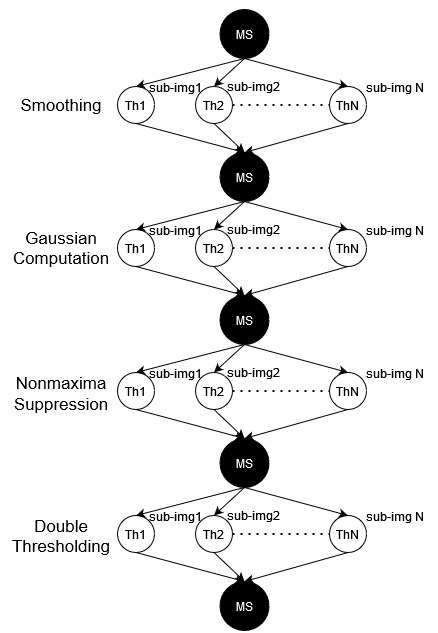
\includegraphics[width=0.8\linewidth]{"./image/pthread_strategy.jpg"}
  \caption{Pthread 平行化流程圖}
  \label{fig:pthread}
\end{figure}

\subsubsection{Load Balancing Problem} \label{load_balancing}

在 Pthread 中,考慮到在 edge linking 階段每個點要搜尋附近是否有可以相連的點,
接著下一個階段再依序檢查上一輪檢查點之附近的點。因為圖片中的邊緣的分布不一定平均,
我們推測經過一段時間後,不同 thread 處理的 pixel 數量會有落差,造成執行時間被單一工作量較大的 thread 拖累。
因此我們嘗試建立一個可以讓各 thread 共享的 queue,在每個 BFS iteration 結束時,
重新統整及分配每一個 thread 要處理的pixel數量,避免工作量不均的狀況。 \\
Load balancing 實作的方式,在每個 iteration 結束前,會有 barrier 讓 thread 暫時被 block 住,
等到所有 thread 執行到此,接著將下一個 iteration 要搜尋的位置 push 到共享的 queue 中。
最後由 master thread 分配各個 thread 下一輪要遍歷的點,不斷重複,直到所有點都被搜尋完。 \\
我們預期這樣的做法可以讓各 thread 的總工作量達到平衡,但同時也會有利用 barrier 所造成的額外負荷,
因此我們會在實驗結果中比較有無使用 load balancing 的差異,並分析其效能。

\subsection{OpenMP}

OpenMP 的實作方式同樣是將沒有資料相依性的 smoothing、gradient calculation、nonmaxima suppression、double thresholding 計算進行平行化,
有資料相依性的 edge linking 步驟則是讓各 thread 維護各自的 queue,並對各自的 queue 進行 BFS 運算。

\subsubsection{Race Condition Problem} \label{race_condition}

在 edge linking 運算中,需要紀錄圖像中各點是否已經被拜訪過,以避免同一點被拜訪多次,
因此我們利用一個各 thread 共享的陣列來記錄各點的拜訪狀態。
在實作時,我們發現若沒有對訪問陣列上鎖,可能會有 race condition,造成同一像素的被拜訪多次,造成不必要的時間浪費,
所以我們提出在這一步利用 \emph{omp\_lock\_t} 對訪問陣列上鎖,確保同一時間只有一個 thread 能夠存取訪問陣列的某一元素。 \\
我們預期上鎖後可以降低對同一像素重複拜訪,不過同時也會有上鎖所造成的額外負荷,
因此我們會在實驗結果中比較有無使用上鎖的差異,並分析其效能。

\subsection{CUDA}

CUDA的實作方式會依據是否具有資料相依性有所不同,由於除了 edge linking 之外的步驟皆沒有資料相依性,
因此這些步驟在 CUDA 進行平行化時,會將單一像素的運算交由一個 thread 進行;
而edge linking需要同時考慮周圍像素的狀態,因此我們利用以下實作方式達到平行化。 \\
在利用 CUDA 實作 edge linking 的平行化時,我們先將圖片切分成若干個子區域,
數量等同於 grid 中 thread block 的個數,各 thread block 會分配到對應其 block ID 的圖片區域進行 edge linking。
在進行 BFS 前,block 中的其中一個 thread 會先將負責區域內的 strong pixel 排入宣告在 shared memory 的 queue 中,
並標記 weak pixel 所在的位置,方便後續進行 BFS 時尋找和 strong 相鄰的 weak pixel。接著 thread block 中的各 thread 會開始進行 BFS,
由於同一 thread block 中的 thread 會進行同步,因此不需要特別考慮 queue 的 race condition 問題,同個 thread block 中也可以達成 load balance。
不過這樣的實作方式會導致各 thread block 負責的區域獨立,忽略橫跨多個子區域的潛在邊緣;
因此我們參照 Luo 等人在\cite{4563088}中提到的兩個改良方式,一為讓子區域相互重疊 1 pixel 的寬度,
讓各 thread block 在初始化 queue 時可以同時考慮相鄰 thread block 的 edge linking 結果;二為重複進行多次 BFS (multi-pass approach),
目的是盡可能找出所有的潛在邊緣。
Figure \ref{fig:cuda}為CUDA 的 edge linking 實作流程圖,可以發現若只進行一次 BFS,會有部分潛在邊緣沒有被找出來,
因此需要進行多次 BFS,才能找出所有的潛在邊緣。
在本次實驗中,我們參照 Luo 等人在\cite{4563088}中的實驗結果,將 BFS 的重複次數設為 4 次,
觀察是否能在低誤差的情況下,找出所有的潛在邊緣。
% 由於能否完整還原潛在邊緣需取決於圖片本身特性和重複次數,
% 因此在進行實驗時我們會確保偵測到的邊緣和實際邊緣的誤差不超過3\%。

\begin{figure}[h]
  \centering
  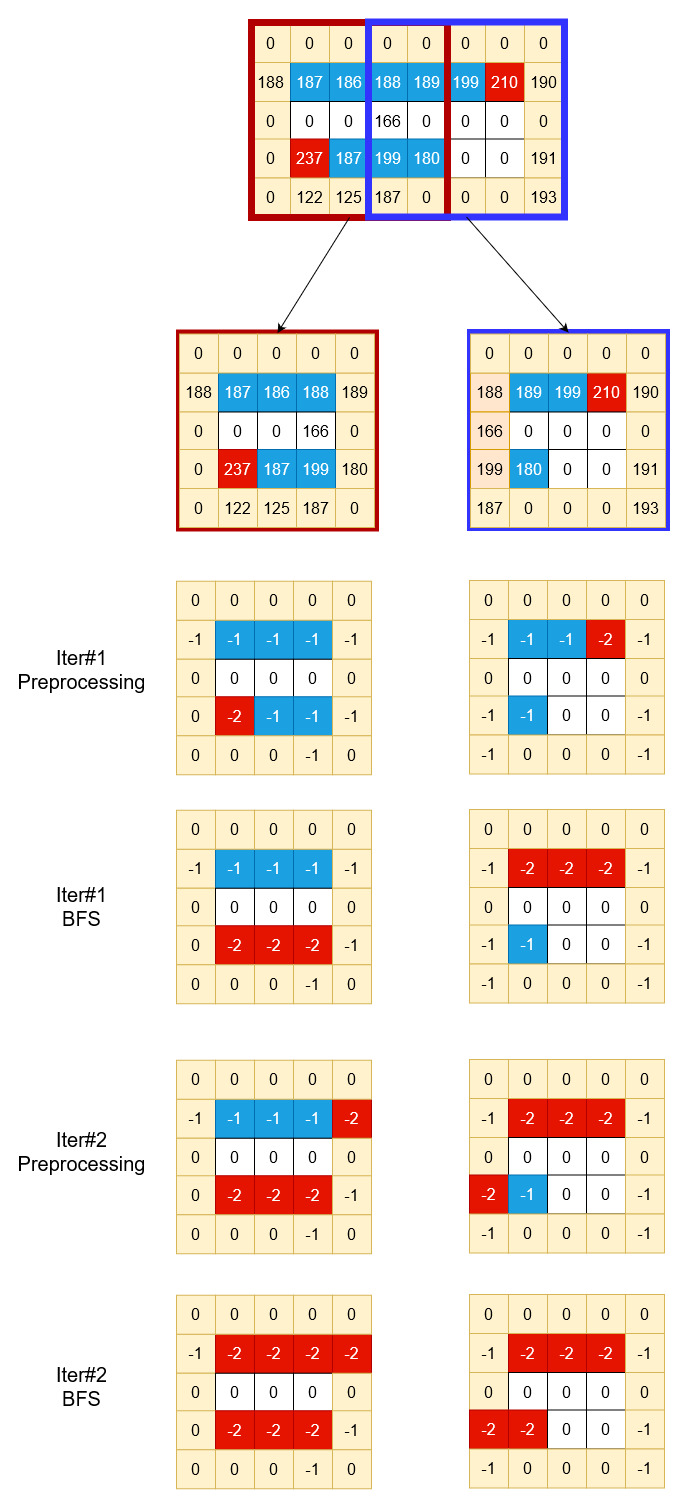
\includegraphics[width=0.8\linewidth]{"./image/cuda_edge_link.jpg"}
  \caption{CUDA Edge Linking 平行化流程圖}
  \label{fig:cuda}
\end{figure}

\section{Experimental Methodology}

基於高效能且支援多種平行化 API 的特性,我們選擇 C++ 作為實作所使用的語言。
在實驗資料部分,我們使用了一張原始大小為 $8192 \times 4951$ 的圖像,並將其縮小另外獲得 $4096 \times 2476$ 、 
$2048 \times 1238$ 、 $1024 \times 619$ 共四張測試圖片進行實驗。在 OpenMP 和 Pthread 的部分,
我們分別使用了 2、3、4 個 thread 進行實驗。
實驗環境為課程所提供的伺服器,詳細規格如下:

\begin{itemize}
  \item CPU: Intel(R) Core(TM) i5-7500 CPU @ 3.40GHz (4core 4thread)
  \item GPU: NVIDIA GeForce GTX 1060 6GB
  \item OS: Ubuntu 20.04.5 LTS
\end{itemize}

\section{Experimental Results}

\subsection{Pthread}

\subsubsection{Speedup and Efficiency with Different Number of Threads}

在Figure \ref{fig:pthread_speedup} 和 Figure \ref{fig:pthread_efficiency}中,
我們可以看到在使用計算大小圖片的情況下,使用不同數量的 thread 時的speedup和 efficiency。
可以發現在相同圖片大小的情況下,使用較多的 thread 時,可以提升speedup,
但是 efficiency會隨著 thread 數量的增加而有些微下降,這是因為在使用較多的 thread 時,
會有較大的 fork-join 開銷,造成 efficiency下降。
比較不同圖片大小的情況下,可以發現在使用較大的圖片時,speedup會比較好,
這是因為大尺寸圖片的總運算量較大,造成 fork-join 開銷對總執行時間的影響較小,
因此可以有較好的speedup和 efficiency。

\begin{figure}[htbp]
  \centering
  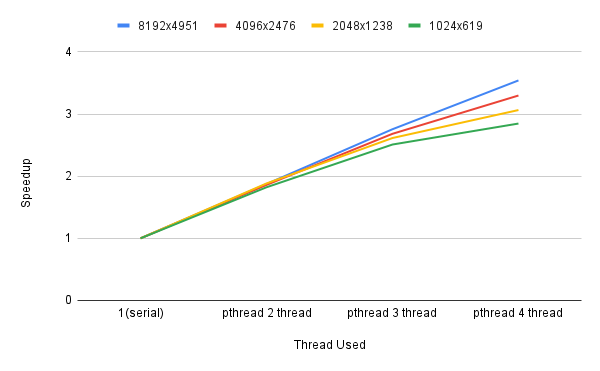
\includegraphics[width=\linewidth]{"./image/pthread_speedup.png"}
  \caption{Pthread 使用不同數量 thread 時的speedup}
  \label{fig:pthread_speedup}
\end{figure}

\begin{figure}[htbp]
  \centering
  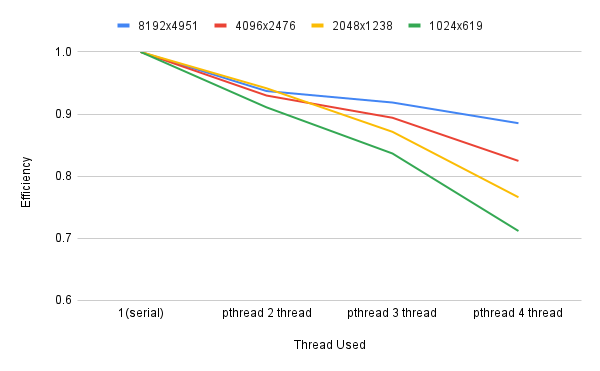
\includegraphics[width=\linewidth]{"./image/pthread_efficiency.png"}
  \caption{Pthread 使用不同數量 thread 時的 efficiency}
  \label{fig:pthread_efficiency}
\end{figure}

\subsubsection{Load Balancing Problem}

在 \ref{load_balancing} 中,我們提出了一個 load balancing 的方法,
來降低各 thread 工作量不均的問題。
最終兩者執行時間如 Figure \ref{fig:pthread_load_balancing}所示,
可以看到不論使用多少 thread ,實作 load balancing 的版本都比較慢,

\begin{figure}[htbp]
  \centering
  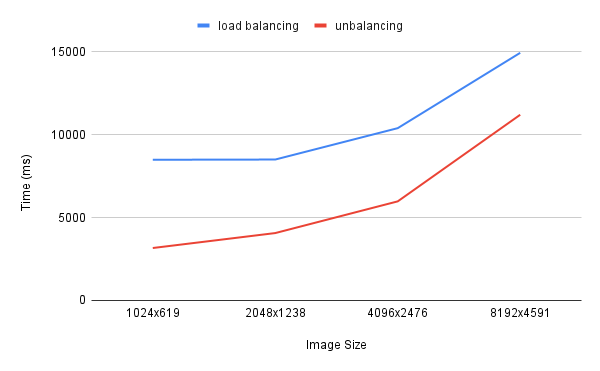
\includegraphics[width=\linewidth]{"./image/pthread_load_balance.png"}
  \caption{Load Balancing 前後執行時間比較}
  \label{fig:pthread_load_balancing}
\end{figure}

根據我們的實驗,前5個 iteration 所佔據的時間,佔據約整體 edge linking 時間的 85\% 以上,
由於起初我們會先將要計算的像素位置平分給所有 thread,因此各 thread 處理的像素數量是差不多的;
而在 edge linking 的中期開始出現分配不均的現象 (如 Figure \ref{fig:pthread_load}) ,
各個thread要處理的pixel數量開始有差異,
但剩餘要處理的像素不多,
即使有分配不均的現象也不會對整體執行時間造成太大的影響;
後半段的分配問題更為嚴重,但執行時間佔據比例已經很小,不足以影響整體執行時間。
且我們發現在加入 load balancing 後,執行時間反而變慢,這是因為在加入 load balancing 後,
各 thread 需要花費額外的時間來進行同步,拖累整體執行時間。

\begin{figure}
  \centering
  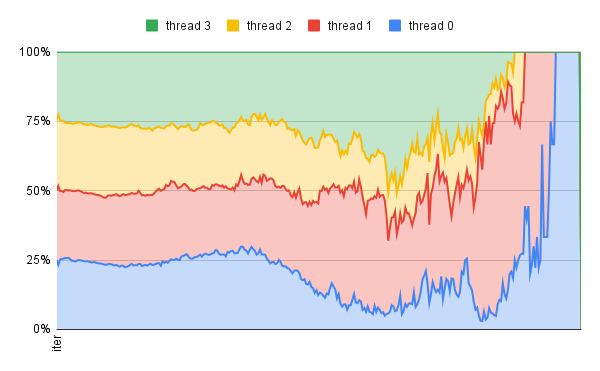
\includegraphics[width=\linewidth]{"./image/pthread_load.png"}
  \caption{各 thread 處理的像素數量}
  \label{fig:pthread_load}
\end{figure}

\subsection{OpenMP}

\subsubsection{Speedup and Efficiency with Different Number of Threads}

在Figure \ref{fig:openmp_speedup} 和 Figure \ref{fig:openmp_efficiency}中,
我們可以看到在使用計算大小圖片的情況下,使用不同數量的 thread 時的speedup和 efficiency。
和 Pthread 的結果相同,可以發現在相同圖片大小的情況下, efficiency會隨著 thread 數量的增加而有些微下降。
且比較不同圖片大小的情況下,可以發現在使用較大的圖片時,speedup會比較好。

\begin{figure}[htbp]
  \centering
  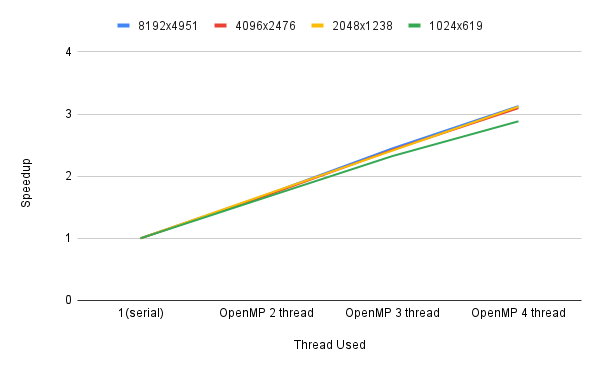
\includegraphics[width=\linewidth]{"./image/openmp_speedup.png"}
  \caption{OpenMP 使用不同數量 thread 時的speedup}
  \label{fig:openmp_speedup}
\end{figure}

\begin{figure}[htbp]
  \centering
  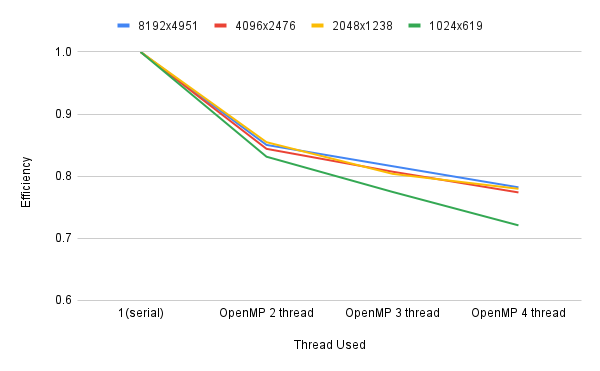
\includegraphics[width=\linewidth]{"./image/openmp_efficiency.png"}
  \caption{OpenMP 使用不同數量 thread 時的 efficiency}
  \label{fig:openmp_efficiency}
\end{figure}

\subsubsection{Race Condition Problem}

在 \ref{race_condition} 中,我們提出藉由對訪問陣列上鎖,
以避免重複拜訪同一像素的方法,來降低執行時間。
我們使用 \emph{omp\_lock\_t} 來對訪問陣列中每一元素上鎖,
並使用 4 個 thread 的 OpenMP 比較有使用 lock 及沒使用 lock 的版本在各類圖片大小時的比較。
由 Figure \ref{fig:openmp_visit_lock} 可以發現,在執行 Edge Linking 的時間上,
有使用 lock 的執行時間在各種尺寸的圖片上都比沒使用 lock 高,圖片尺寸越大,
執行時間的差距比例也越大 ,進一步去統計總共拜訪的節點數,
由 Figure \ref{fig:openmp_visit_count} 中可以看到,
各尺寸的圖片上的拜訪節點數相差無幾,
沒使用 lock 時,拜訪的節點數僅增加不到 1\%。從這些結果可以發現,
因為 race condition 所造成的重複拜訪節點數沒有預期中的那麼多,
且因拜訪節點後需要做的計算量極少,所以重複拜訪的成本低於使用 lock 的成本,
所以使用 lock  efficiency反而較慢。

\begin{figure}
  \centering
  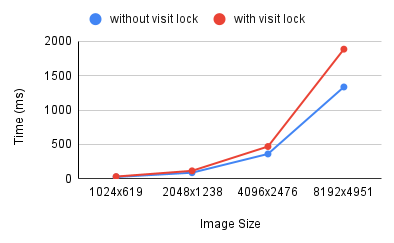
\includegraphics[width=\linewidth]{"./image/openmp_visit_lock.png"}
  \caption{有無使用 Lock 的執行時間比較}
  \label{fig:openmp_visit_lock}
\end{figure}

\begin{figure}
  \centering
  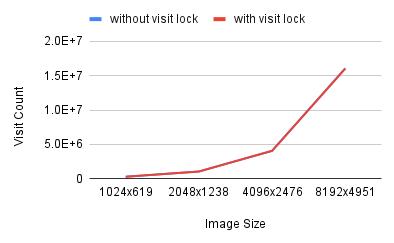
\includegraphics[width=\linewidth]{"./image/openmp_visit_count.png"}
  \caption{有無使用 Lock 的總拜訪節點數比較}
  \label{fig:openmp_visit_count}
\end{figure}

\subsection{All Models}

在 Figure \ref{fig:all_model} 和 Table \ref{tab:all_model} 中,
我們可以看到在計算不同大小圖片的情況下,
使用不同的平行化方法時的speedup。\\
首先,CED 中的大部分都是各個像素的獨立計算,
因此在表中可以看到各模型上在大尺寸圖片上的speedup都比較好,
而在小尺寸圖片上的speedup則不明顯。\\
同樣為利用 CPU 進行平行化,Pthread 和 OpenMP 在各尺寸圖片上的speedup相差不大,
但由於 Pthread 可以更細緻地控制每個 thread 的行為和同步機制,
因此整體上 Pthread 的speedup會比 OpenMP 稍微好一些。\\
CUDA 的實驗結果相較其他兩種平行化方法,在小張圖片的speedup上較為不明顯,
我們推測原因為整體運算量太小,因此搬運圖像資料的時間成本依舊在總時間中佔有一定比例,
這樣的因素導致 CUDA 的speedup在小圖像上較為薄弱。隨著實驗圖像越來越大,
搬運資料的時間成本所佔比例也越來越低,導致CUDA在 speedup 上的優勢也越來越明顯。
由於是將單一像素的運算交由單一 thread 進行,因此可以視為整張圖像的運算是同時進行的,
這和 Pthread 以及 OpenMP 此類利用 CPU 少量核心進行平行化的方法有決定性的差異。

\begin{figure}[htbp]
  \centering
  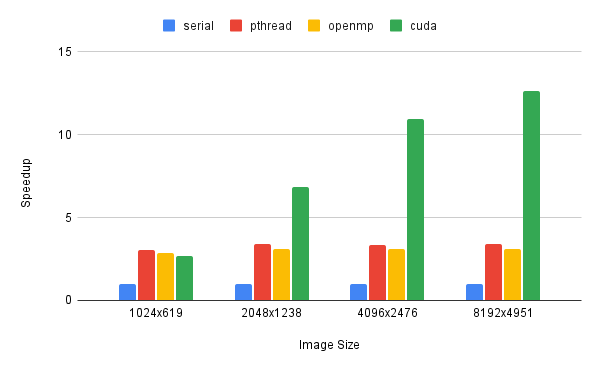
\includegraphics[width=\linewidth]{"./image/all_model.png"}
  \caption{各模型在不同尺寸照片下的speedup}
  \label{fig:all_model}
\end{figure}

\begin{table}[htbp]
  \centering
  \begin{tabular}{|c|c|c|c|c|}
  \hline
  \multirow{2}{*}{Model} & \multicolumn{4}{c|}{Speedup} \\ \cline{2-5} 
                         & 1024x619    & 2048x1238   & 4096x2476   & 8192x4951  \\ \hline
  Pthread                & 3.039       & 3.386       & 3.355       & 3.433      \\ \hline
  OpenMP                 & 2.883       & 3.118       & 3.095       & 3.128      \\ \hline
  CUDA                   & 2.691       & 6.873       & 10.973      & 12.621     \\ \hline
  \end{tabular}
  \caption{各模型在不同尺寸照片下的speedup}
  \label{tab:all_model}
\end{table}

\section{Related Work}

Gonzalez等人在 \cite{gonzalez2018digital} 中提及了 Canny 演算法的概念,
並介紹了每個步驟中的過程並給出了一些實做細節上的選擇,比如 Smoothing 中 filter 的選擇,
或是 Gradient Computation 中計算 Gradient 的方式,但沒有提及如何使用平行化加速演算法的執行,
所以我們接下來將介紹其他將此演算法利用平行化加速的研究。 \\
Cheikh等人在\cite{6328953}中提出了兩種平行化的策略,
分別為loop-level parallelism和domain decomposition;
loop-level parallelism是將個步驟中可獨立運行的迴圈交由多個thread執行,
但由於需要反覆進行fork-join,因此會有額外的開銷,
且會因為計算全域資料而失去資料局部性(data locality);
domain decomposition是將資料本身進行分割再交由thread完成各分區的各項步驟,
雖然domain decomposition沒有前述loop-level parallelism的缺陷,
但需要選擇適合的資料分割方式來降低平行化時的相依性來達到最佳效能。
Cheikh等人將兩種方式在多核CPU和GPU上進行實驗,
發現loop-level parallelism在GPU上運行無serial的程式時可以達到很好的speedup,
而domain decomposition適合在CPU上針對大型資料的運算進行平行化;
最後他們結合了兩種平行化策略,發現結合後的speedup和擴展性相比於兩種平行化策略,
在CPU和GPU的表現都更好,因此我們在針對CED的平行化策略上,
也採取了結合loop-level parallelism和domain decomposition的方式,預期可以達到最好的成果。 \\
Luo等人在在\cite{4563088}中嘗試以CUDA 框架對Canny Edge Detection進行平行化,
並且提到過往在Canny Edge Detection中hysteresis labeling connected component part的平行化處理較少,
因為此步驟平行化需要non-local memory,導致 speedup 與 efficiency 顯著降低。
論文中使用GPU在處理pixel-wise operations有較高效率的特性來加速non-maximum suppression、
hysteresis and connected components等部分,並引入Apron pixels的機制來讓所有像素可以在卷積中操作。
實驗結果顯示,與CPU版本的實作相比,隨著圖片大小而有1.6X ~ 3.8X不等的speedup。
另外GPU版本的hysteresis為了同步不同thread block間的運算使用了multi-pass approach,
導致GPU運算速度降低,佔據75\%以上的運行時間。

\section{Conclusion}

經過我們利用三種平行化方法的實驗後,我們可以發現 Pthread與 OpenMP speedup相差不大,
但 Pthread 平均運行時間會略短於 Openmp。
不過 Openmp 具有撰寫容易的特性,
不須太大幅度更動原先程式的架構即可完成平行化;
而Pthread則需要自行分割程式邏輯,獨立出要平行部分。
在比較不同 thread 數量的實驗中,由於我們演算法的特性計算具有較高的獨立性,
因此speedup大致上隨著使用的 thread 數量等比下降,在 2 ~ 4 個 thread 都維持在 0.7 以上的 efficiency。
此外,lock、mutex、barrier 等同步機制所消耗的時間是相對高的,
即使可以減少演算法中不必要的計算量,
但若減少的計算量不足以彌補同步機制所消耗的時間,
仍然會增加整體的執行時間。
在CUDA上,由於運算單元更多,可以對各個像素平行化處理,
因此speedup會更明顯;但因需要額外的資料搬移,在小圖的speedup上並不明顯。


% \subsection{Parallelization Strategies}

% 綜上所述,我們會將CED的平行化分為For Loop Parallelism和Data Decomposition兩部分,
% 前四步驟為將各像素的運算交由thread進行加速,Hysteresis Edge Linking的部分則是將圖像分割,
% 讓thread對各分區進行運算。流程圖如圖\ref{fig:diagram}所示。

% \begin{figure}[h]
%   \centering
%   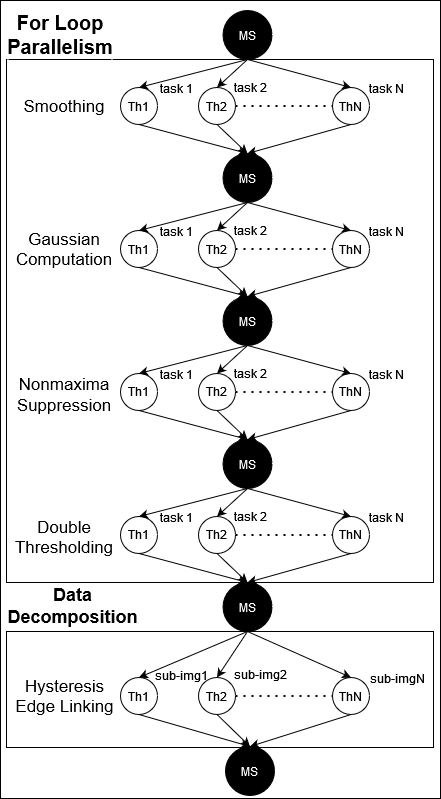
\includegraphics[width=\linewidth]{parallel_diagram.png}
%   \caption{Parallel Strategies and Flow Chart of Canny Edge Detection Parallelism}
%   \label{fig:diagram}
% \end{figure}

% \section{Language Selection}

% 我們的程式語言使用 C++。因為C++ 是編譯型語言,在執行之前會被轉換為機器碼,
% 使C++ 較為快速和高效;且C++ 提供控管記憶體的方式,給予一定靈活與設計空間;
% 同時C++ STL提供多種 API 來支持平行化,包括std::future、std::atomic等。
% 並且可使用其他框架來支持平行化,如OpenMP、CUDA、OpenCL。

% \section{Statement of Expected Results}

% 針對CED的平行化,我們提出了數個理論並希望可以藉由實驗來觀察並驗證其正確性。

% \subsection{圖像大小 vs. 加速效果}

% 我們會針對不同大小的圖像進行CED的平行化測試,由於CED的多個步驟都是針對各像素進行運算,
% 可以推斷圖像大小等同於運算量的多寡,因此我們預期大張圖像的加速效果會優於小張圖像的加速效果。

% \subsection{平行化程式的擴展性}

% 藉由不同的thread數量進行實驗,我們可以計算在運行多個thread的情況下是否可以達到預期的加速效果。
% 因為Hysteresis Edge Linking步驟需要對thread進行同步,
% 因此我們認為該步驟會在增加thread的同時增加同步所需要的開銷,從而限制加速的效果。

% \subsection{Pthread vs. OpenMP}

% 雖然Pthread和OpenMP同樣使用CPU進行加速,但針對thread的行為部分,
% Pthread是開發者自定義而OpenMP是取決於編譯器,因此我們認為Pthread的加速效果會優於OpenMP。

% \subsection{Pthread vs. CUDA}

% CUDA雖然使用GPU進行加速,但需要將資料在記憶體和GPU之間進行搬運,從而增加搬運的開銷;
% 因此我們會利用小張圖像測試Pthread和CUDA的加速效果,
% 觀察搬運開銷是否會在運算小張圖像時降低CUDA的加速效果。

% \subsection{Comparison of All Method}

% 最後我們會利用1920*1080的圖像對不同加速方法進行測試,觀察並比較不同方法之間的加速效果。

%%
%% The next two lines define the bibliography style to be used, and
%% the bibliography file.
\bibliographystyle{ACM-Reference-Format}
\bibliography{sample-base}

\end{document}
\endinput
%%
%% End of file `sample-xelatex.tex'.
